\section{2. Euclidean Space}
% **************************

\subsection{Properties of vectors}
% ================================

Dot product, norm and distances. The dot product of two vectors \textbf{A} and
\textbf{B} can be thought as the prodcut of their magnitude times the angle between
them:

$$\mathbf{A} \cdot \mathbf{B} = \|\mathbf{A}\| \cdot \|\mathbf{B}\|cos(\theta)$$

Since $cos(\pi/2) = 0$, if the two vectors are orthogonal their dot product is
0. For example $\left[\begin{matrix}2\\0\end{matrix}\right] \cdot \left[\begin{matrix}0\\2\end{matrix}\right] = 0$

\subsubsection{Exercise 2.1.1}
% ----------------------------

Evaluate

\begin{verbatim}
import matplotlib.pyplot as plt

u= Matrix(2, 1, [-1, 3])
v= Matrix(2, 1, [2, 1])

plt.text(float(u[0])+0.2, float(u[1]), 'u', fontsize= 30, color= 'r')
plt.text(float(v[0])-0.2, float(v[1]), 'v', fontsize= 30, color= 'r')
plt.arrow(0, 0, float(u[0]), float(u[1]), lw= 3, color= 'b', head_width=0.05)
plt.arrow(0, 0, float(v[0]), float(v[1]), lw= 3, color= 'b', head_width=0.05)
plt.xlim((-1.1, 3.1))
plt.ylim((-1.1, 3.1))
plt.grid()
plt.savefig('figs/ex2_1_1.pdf')
plt.close()
\end{verbatim}

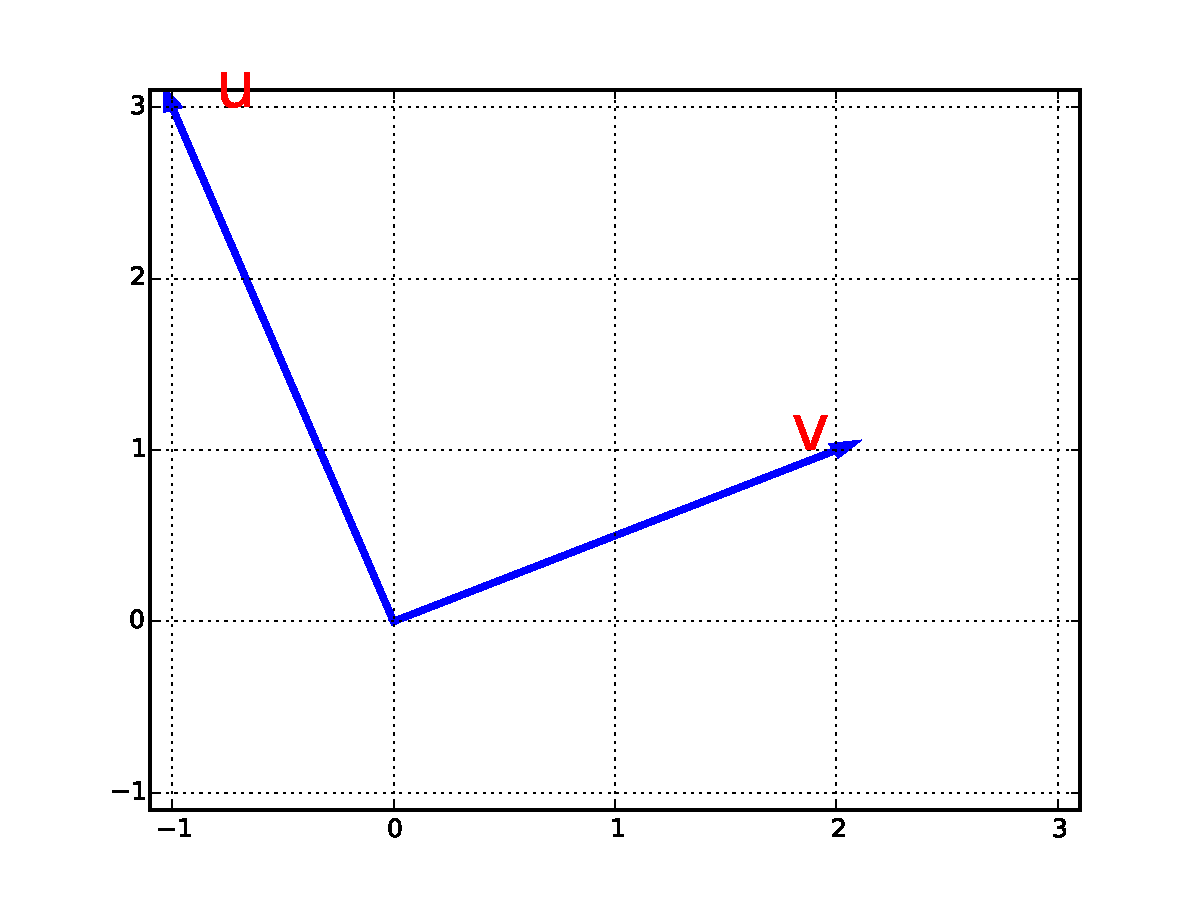
\includegraphics[width=\linewidth]{figs/ex2_1_1.pdf}

\begin{verbatim}
u.dot(v) # 1
v.dot(u) # 1
u.dot(u) # 10
v.dot(v) # 5

u.norm()            # sqrt(10)
u.norm()**2         # 10
v.norm()            # sqrt(5)
v.norm()**2         # 5
(u + v).norm()**2   # 17
(u - v).norm()      # sqrt(13)
\end{verbatim}

\subsubsection{Exercise 2.1.3}
% ----------------------------
Evaluate for
$\mathbf{u} = \left[\begin{matrix}-1\\2\\5\\-3\end{matrix}\right]$ and
$\mathbf{v} = \left[\begin{matrix}2\\-3\\-1\\5\end{matrix}\right]$

\begin{verbatim}
u= Matrix(4, 1, (-1, 2, 5, -3))
v= Matrix(4, 1, (2, -3, -1, 5))
\end{verbatim}

\textbf{Dot product}:

\begin{verbatim}
v.dot(u)    # -28
u.dot(v)    # -28  
v.dot(v)    # 39
u.dot(u)    # 39
\end{verbatim}

Note that commutative property hold. NB \textbf{\texttt{u * v}} raises \texttt{\textcolor{red}{ShapeError: Matrices size mismatch.}}

\textbf{Norm} (\emph{symbol}: $\|u\|$, $\|u + v\|$, $\|u\|^2$, etc)

\begin{verbatim}
u.norm()            # sqrt(39)
u.norm()**2         # 39
v.norm()            # sqrt(39)
v.norm()**2         # 39
(u + v).norm()**2   # 22
\end{verbatim}

\textbf{Distance} $d(u, v) = \| u - v \|$

\begin{verbatim}
(u - v).norm() # sqrt(134)
(v - u).norm() # sqrt(134)
\end{verbatim}

\subsubsection{Exercise 2.1.6}
% ----------------------------

Plot and compute for $\mathbf{u} = \left[\begin{matrix}7\\-2\end{matrix}\right]$
and $\mathbf{v} = \left[\begin{matrix}-5\\3\end{matrix}\right]$

$$\|\mathbf{u} + \mathbf{v} \| = \sqrt{5}$$
and
$$d(\mathbf{u}, \mathbf{v}) = \|\mathbf{u} - \mathbf{v} \| = 13$$

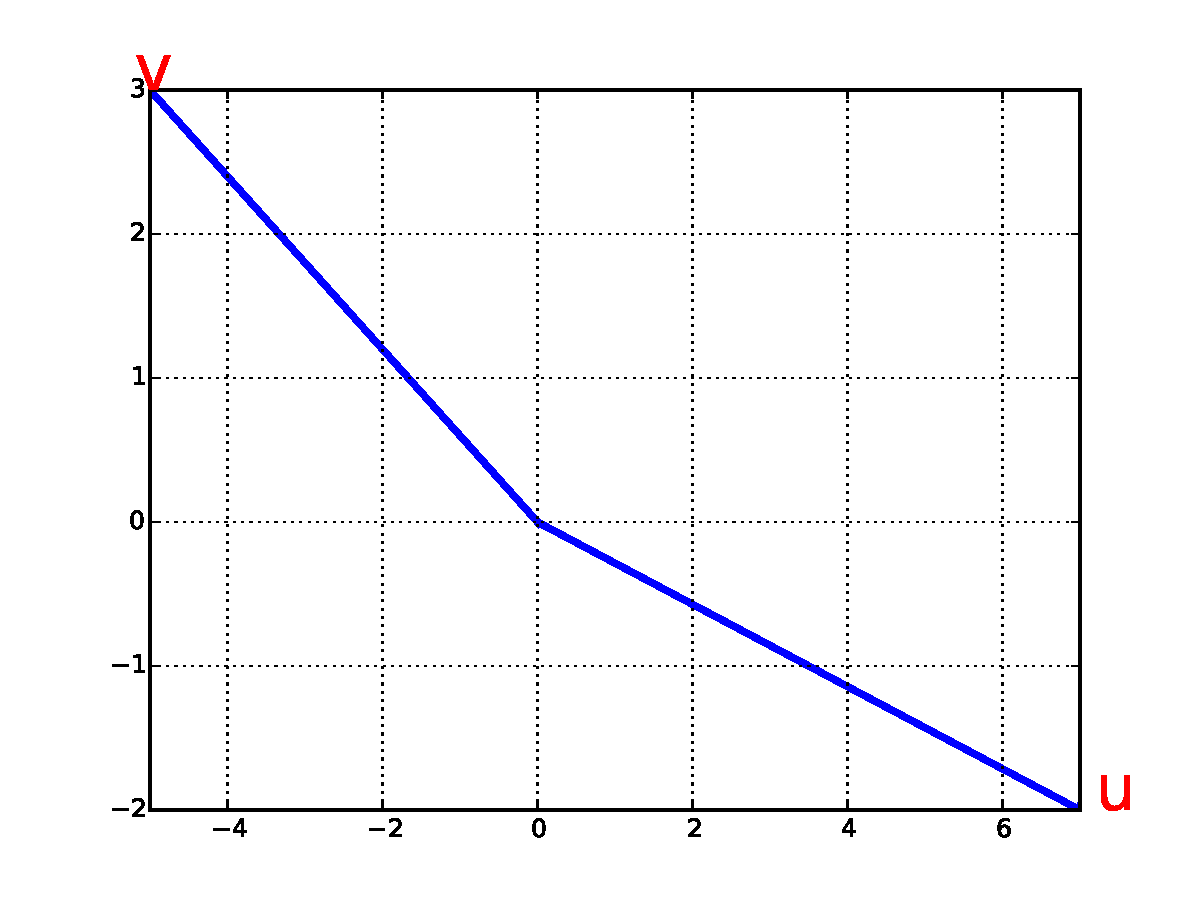
\includegraphics[width=\linewidth]{figs/ex2_1_6.pdf}

\begin{verbatim}
u= Matrix(2, 1, [7, -2])
v= Matrix(2, 1, [-5, 3])

plt.text(float(u[0])+0.2, float(u[1]), 'u', fontsize= 30, color= 'r')
plt.text(float(v[0])-0.2, float(v[1]), 'v', fontsize= 30, color= 'r')
plt.arrow(0, 0, float(u[0]), float(u[1]), lw= 3, color= 'b', head_width=0.05)
plt.arrow(0, 0, float(v[0]), float(v[1]), lw= 3, color= 'b', head_width=0.05)
plt.xlim((-5, 7))
plt.ylim((-2, 3))
plt.grid()
plt.savefig('figs/ex2_1_6.pdf')
plt.close()

(u + v).norm() # sqrt(5)
(u - v).norm() # 13
\end{verbatim}


\subsection{Further Properties of Vectors}
========================================

\subsubsection{Exercise 2.2.1}

Find the angle between vectors. The angle is

\begin{equation}\label{eq:uv_angle}
\theta = \arccos(\frac{\mathbf{u} \cdot \mathbf{v}}
{\|\mathbf{u}\| \cdot \|\mathbf{v}\|})
\end{equation}

In \sympy

\begin{verbatim}
def uv_angle(u, v):
    theta= acos(u.dot(v) / (u.norm() * v.norm()))
    return theta
\end{verbatim}

\begin{verbatim}
u= Matrix([1, 1])
v= Matrix([0, 1])
uv_angle(u, v) # pi/4

# As degree:
uv_angle(u, v) * 180/pi # 45

u= Matrix([-1, 2, 3])
v= Matrix([sqrt(2), 1/sqrt(2), -1])
uv_angle(u, v) * 180/pi # ~115 deg
\end{verbatim}

\subsubsection{Exercise 2.2.4}
% ----------------------------
Determine the vector of $k$ so that the vectors are orthogonal to each other.

We want to set the angle between vector equal to 0, \emph{i.e.} Eq. \ref{eq:uv_angle} = 0.

\begin{verbatim}
k= symbols('k', real= True)
u= Matrix([-1, 5, k])
v= Matrix([-3, 2, 7])

eq= Eq(u.dot(v) / (u.norm() * v.norm()) , cos(pi/2))
sol= solve(eq)

# Check
u.subs(k, sol[0]).dot(v) == 0 # True
\end{verbatim}

\subsubsection{Exercise 2.2.6}
% ----------------------------

A vector is normalized by dividing it by its norm. A normalized vector is called
\textbf{unit vector}. In \sympy normlaize with:

\begin{verbatim}
def norm_u(u):
    return u / u.norm()
\end{verbatim}

Determine the value of $k$ so that $\mathbf{\hat{u}} = (1/\sqrt{2}\ 1/2\ k)^T$.

For \textbf{u} to be unit vector, its norm must equal 1. So $\mathbf{\|u\|} = \sqrt{\left\lvert{k}\right\rvert^{2} + 0.75} = 1$.
Solved for $k= \pm 1/2$.

\begin{verbatim}
u= Matrix([1/sqrt(2), 1/2, k])
eq= Eq(u.norm(), 1)
ksol= solve(eq) # [-0.5, 0.5]
\end{verbatim}

\subsubsection{Exercise 2.2.12: Support vector machine}
% -----------------------------------------------------

Find the 

% \subsection{Linear Independence}
% ==============================

% \subsection{Basis and Spanning Set}
% =================================

